\documentclass[a4paper]{scrreprt}
\setcounter{tocdepth}{3}
\setcounter{secnumdepth}{3}

\usepackage[german]{babel}
\usepackage[utf8]{inputenc}
\usepackage[T1]{fontenc}
\usepackage{ae}
\usepackage{graphicx}


\begin{document}
\title{Entwurf}
\author{Fangzhou Bian, Kathrin Blum, Matthias Bruns, \\Leonhard Duda, Tan Grumser, Yuguang Lin}
\maketitle
%\Footnote für Fußnoten
% Platzierung des Inhaltsverzeichnisses
\tableofcontents



\chapter{Einleitung}

\chapter{Grobentwurf}
\section{Systemarchitektur}
Die App MensaMeet wird als Client-Server Anwendung umgesetzt. Clients fordern Dienste an, welche vom zentralen Server bereitgestellt werden. Dazu hat jeder Client, nachdem er sich einmal registriert hat, eine eindeutige User-ID. Der Server verwaltet eine Datenbank, in welcher User- und Gruppeninformationen gehalten werden. 
Die Client-Seite der Anwendung wird mithilfe der MVVM (Model-View-Viewmodel) Architekur umgesetzt.
Die Server-Seite mithilfe der MVC (Model-View-Control) Architektur.

\subsection{Client}
Die Client Seite bedient sich der MVVM Architektur. Die View dient zum anzeigen von Daten, sie beinhaltet alle grafischen Elemente, stellt also die GUI dar. Im Model werden die Daten gehalten und Funktionen zur Manipulation der Daten bereitgestellt.
Das Viewmodel enthält die Darstellungslogik für die View und kapselt sie von der Anwendungslogik, die sich im Model befindet, ab.
View und Viewmodel sind durch Databinding nur lose gekoppelt. Dadurch kann die View problemlos ausgetauscht werden bzw. können mehrere verscheidene Views (z.b. angepasst an Tablet, Desktop,...) zum selben Viewmodel existieren.
Das Datainding kann als bidirektionaler Beobachter verstanden werden. Die lose Kopplung verbessert die Testbarkeit.

\subsection{Server}
Für die Server Seite wird die MVC Architektur verwendet.
Das Model ist für die Datenhaltung zuständig und beinhaltet/verwaltet eine Datenbank.  (In unserem Fall wird MySQL verwendet, als Kommunikationsschnittstelle zwischen der Datenbank und den Controllern wollen wir JPA mit Hibernate benutzen).
View ist durch eine Schnittstelle gegeben, über die der Server Anfragen des Client empfängt und an den Controller delegiert. Der Controller führt diese Anfragen durch, indem er angefordere Daten aus dem Model holt oder neue Daten einfügt bzw Daten anpasst.
\section{Systemkomponenten}
\section{Komponentenbeschreibung}
\subsection{Client}
\subsection{Server}


\chapter{Feinentwurf}
\section{Klassen des Clients}
\subsection{Klassendiagramm}

\subsubsection{Muster}

\section{Klassen des Server}
\subsection{Klassendiagramm}
\subsection{package.edu.kit.mensameet.models}
\subsubsection{Class User}
\subsubsection*{Beschreibung}
Diese Klasse beschreibt einen User 

\subsubsection*{Konstruktor}
public User(String name, String password)

\subsubsection*{Methoden}
\begin{addmargin}[25pt]{0pt}

\subsubsection*{Paramter}
\begin{itemize}
\item
\item
\item
\end{itemize}

\subsubsection*{Rückgabewert}
\end{addmargin}
\subsubsection{Muster}


\chapter{Datenstrukturen}

\chapter{Dynamische Modelle}
\section{Aktivitätsdiagramm}

\section{Sequenzdiagramm}
\subsection{Registrieren}
\begin{center}
	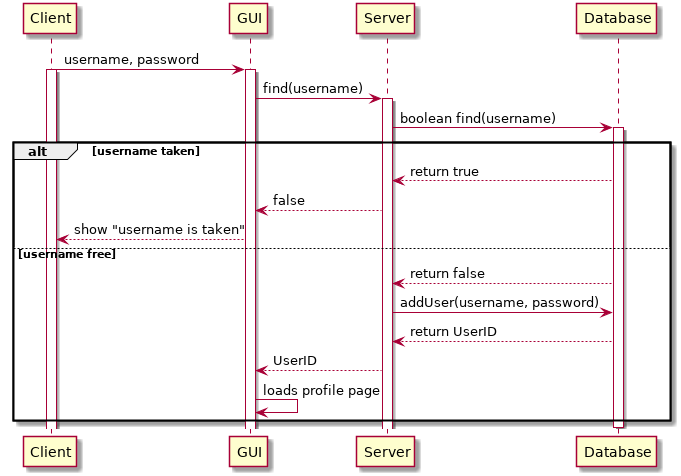
\includegraphics[width=0.93\textwidth]{Sequenzdiagramme/Registration.png}
\end{center}
\subsection*{Beschreibung}
Der Client öffnet zum ersten mal die Anwendung MensaMeet und sieht den Registrierungsbildschrim. Dort soll er einen Nutzernamen und ein Passwort eingeben. Da der Nutzername eindeutig sein muss, wird beim Server angefragt, ob dieser Nutzername schon vergeben ist. Dazu wird in der Datenbank nach diesem Nutzernamen gesucht. Ist der Name schon vergeben, so wird er zurückgegeben und der Client erhält die Meldung "Dieser Nutzername ist bereits vergeben".
Falls der Nutzername noch nicht vergeben ist, wird er nun der Datenbank hinzugefügt und dem Client wird die erfolgreiche Durchführung übermittelt. Der Client wird nun auf die nächste Seite geleitet.
\newpage
\subsection{Mensalinien wählen}
\begin{center}
	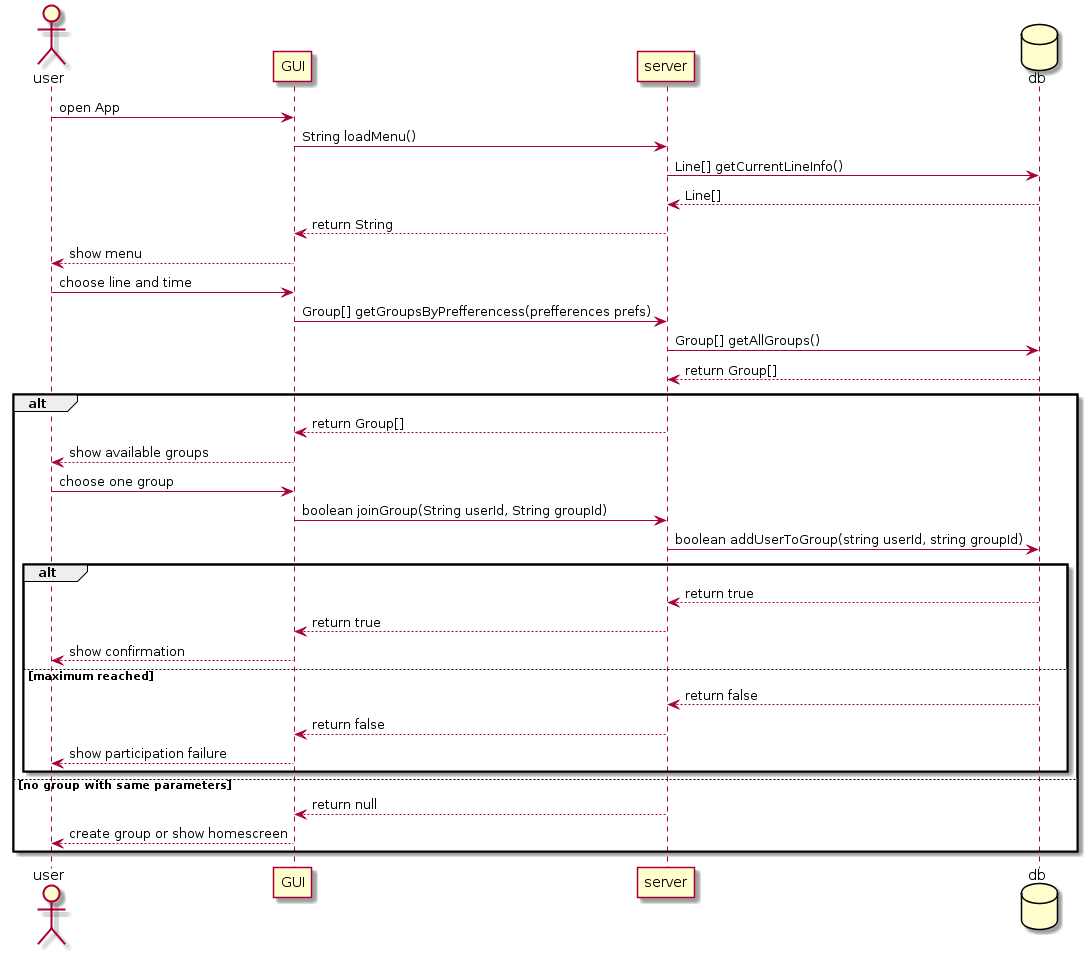
\includegraphics[width=0.93\textwidth]{Sequenzdiagramme/chooseLineAndTimeSD.png}
\end{center}
\subsection*{Beschreibung}
Der Client öffnet die Anwendung (die Registrierung ist bereits erfolgt). Nun soll der Client als Scrolldown-menü die Mensalinien mit ihrem jeweiligen Angebot zu sehen kriegen (Dies ist der "HomeScreen"). Dazu werden die Mensadaten über den Server von der Datenbank angefragt, aufbereitet und dem Client übermittelt. Dieser kann nun die Linien anklicken an denen er gern essen möchte. Danach stellt er das für ihn geeignete Zeitintervall ein. Diese Daten werden dem Server übermittelt, welcher in der Datenbank nach passenden Gruppen sucht und diese zurückgibt. Der Client kann sich die Gruppen anschauen und einer davon beitreten. Beim Versuch beizutreten wird dem Server die UserID und GroupID übermittelt. Es wird überprüft ob die Gruppe bereits voll ist, ist dies der Fall, erhält der Client eine Fehlermeldung und gelangt wieder zur Gruppenübersicht. Ist noch Platz in der Gruppe, wird die Datenbank aktualisiert und dem Client der Beitritt bestätigt. 
Falls keine Gruppen passend zu den Angaben des Clients gefunden wurde, erhält der Client eine passende Meldung und kann entweder zurück zum HomeScreen oder selbst eine Gruppe erstellen.


\subsection{Gruppe beitreten}
\begin{center}
	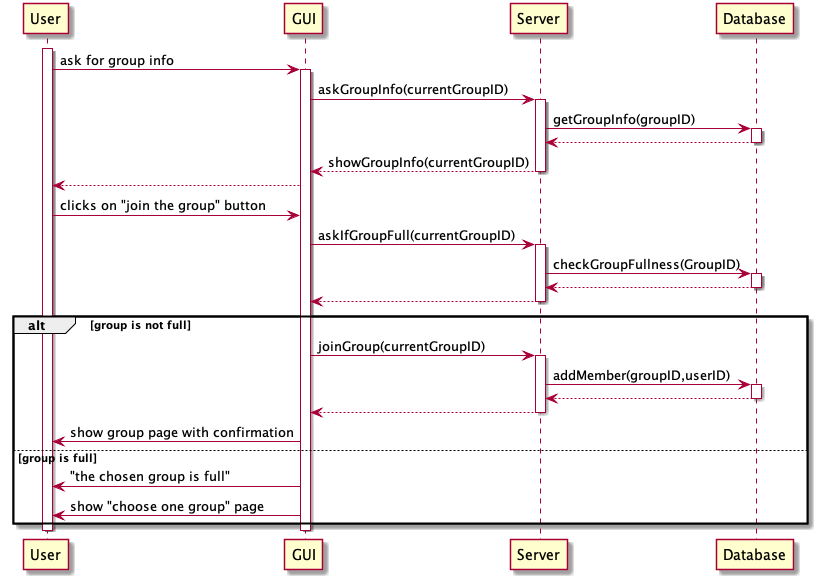
\includegraphics[width=0.93\textwidth]{Sequenzdiagramme/SD_checkInfo&joinGroup.png}
\end{center}

\subsection*{Beschreibung}
Der Client bekommt, passend zu seinen ausgewählten Linien und seinem eingestellten Zeitintervall, Gruppen in einem Scrolldown-menü angezeigt.
Er klickt eine Gruppe an, um mehr Informationen zu ihr zu sehen. Dazu wird an den Server eine Anfrage mit der GroupID gesendet. Der Server sucht die Gruppe in der Datenbank und übermittelt die angefragten Daten dem Client. Dieser drückt nun auf "Beitreten". Nun wird dem Server die UserID und GroupID übermittelt. Er prüft in der Datenbank ob die Gruppe bereits voll ist. Ist dies der Fall, erhält der Client eine Fehlermeldung : "Deine gewählte Gruppe ist bereits voll" und gelangt wieder zur Gruppenübersicht. Ist noch Platz in der Gruppe, wird die Datenbank aktualisiert und dem Client der Beitritt bestätigt. 

\newpage
\subsection{Gruppe erstellen}
\begin{center}
	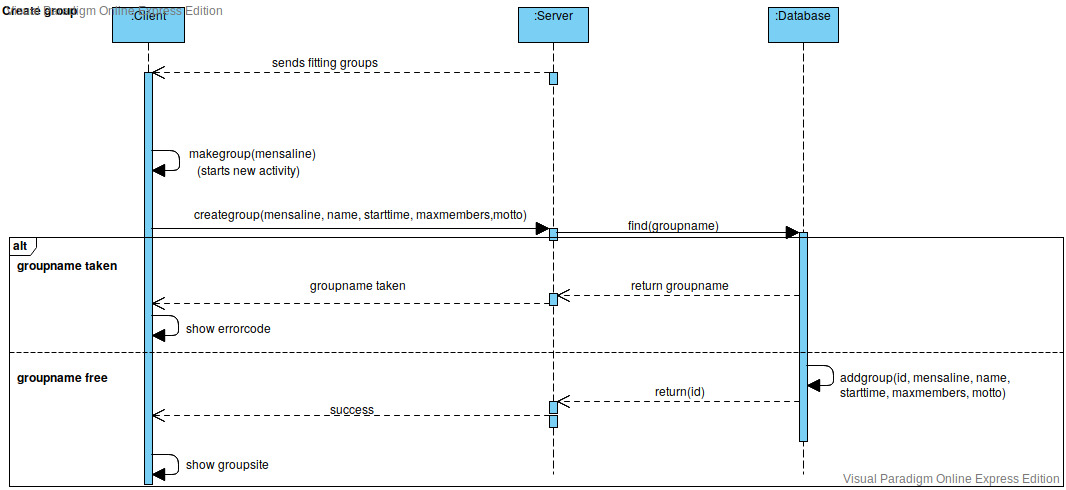
\includegraphics[width=0.93\textwidth]{Sequenzdiagramme/CreateGroup.jpg}
\end{center}
\subsection*{Beschreibung}
Der Client entscheidet sich, selbst eine Gruppe zu erstellen. Er stellt dazu die erforderlichen Gruppenparameter(Gruppenname, Mensalinie, Startzeit, Motto, Maximale Mitgliederzahl) ein. Nun erhält der Server die Anfrage mit diesen Paramtern eine neue Gruppe anzulegen. Da der Gruppenname eindeutig sein muss, wird in der Datenbank nach einer Gruppe mit selben Namen gesucht. Gibt es eine, erhält der Client eine entsprechende Fehlermeldung und kann die Parameter bearbeiten. Gibt es noch keine Gruppe mit diesem Namen wird die Gruppe in der Datenbank angelegt und dem Client die erfolgreiche Gruppengründung bestätigt und ihm wird die Detailansicht seiner Gruppe angezeigt.

\newpage
\subsection{Gruppe verlassen}
\begin{center}
	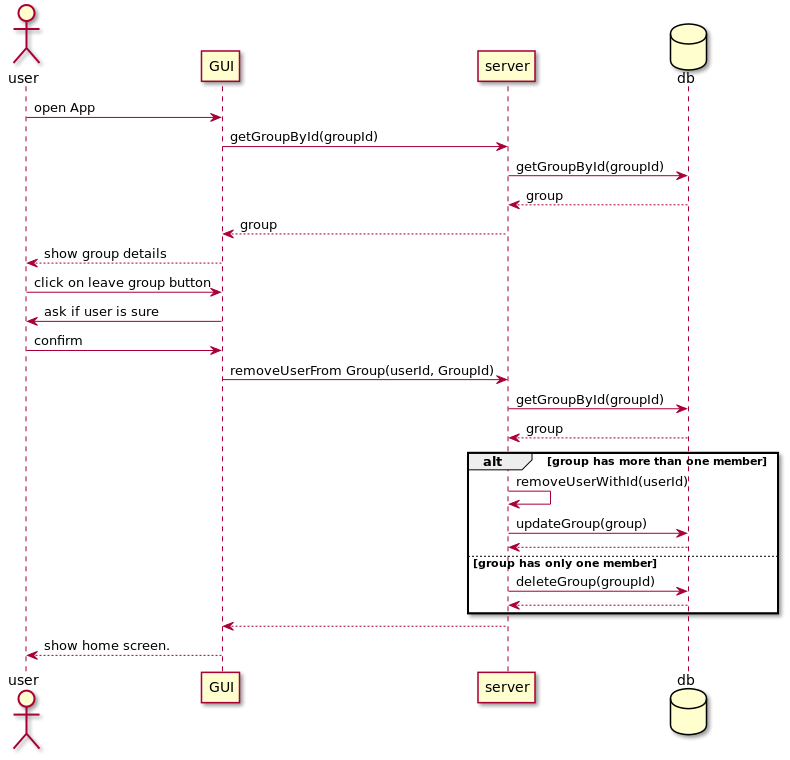
\includegraphics[width=0.93\textwidth]{Sequenzdiagramme/leaveGroupSD.png}
\end{center}

\subsection*{Beschreiung}
Der Client öffnet die App MensaMeet. Da er bereits Mitglied einer Gruppe ist, wird ihm die Detailansicht seiner Gruppe angezeigt.
In dieser Ansicht ist ein Button "Gruppe verlassen". Der Client drückt diesen Button und muss seine Entscheidung bestätigen. Für den Austritt wird dem Server die UserID und GroupID übermittelt. Der Server sucht via GroudID die Gruppe in der Datenbank um sie zu aktualisieren. Der Client wird aus der Gruppe entfernt und die Mitgliederzahl der Gruppe überprüft. Ist diese nun bei 0, so wird die Gruppe aus der Datenbank gelöscht.
Der Client erhält in beiden Fällen die Bestätigung zum Austritt aus der Gruppe und wird wieder zum HomeScreen geleitet.


\chapter{Änderungen zum Pflichtenheft}

\chapter{Glossar}

\chapter{Anhang}

\end{document}
